\subsection{Datasets}

\subsubsection{Synthetic}\label{sec:dataset_synthetic}

The first dataset is a manually created scene in Blender\cite{blender} demonstrating the principle effects of rotation and translation on the conversion results.
Both rotation and translation are done in isolation as well combined.
The scene consists of a sphere, a cylinder, a cube-like object with additional edges of different smootheness and a complex monkey head in a room (Figure~\ref{fig:blender_scene}).
The camera movement is rendered as an animation and the depth buffer of each frame is extracted and used as depth image.
The camera matrix is calculated from the rendering settings and its parameters are provided in Table~\ref{tab:blender_intrinsic}.
The total animation consists of 211 images and no noise is applied to the depth image (example images in Appendix~\ref{sec:synthetic_conversions}).
\begin{figure}[H]
\CenterFloatBoxes%
\begin{floatrow}
    \btabbox{%
    \renewcommand{\arraystretch}{1.2}%
    \setlength{\tabcolsep}{1em}%
    \begin{tabular}{rc}
    \toprule
    \textbf{Parameter} & \textbf{Blender Camera} \\
    \midrule
    Principle  & render/pinhole \\
    Resolution & 1080 $\times$ 1080\,px \\
    $f_x$, $f_y$ & 2220.0, 2220.0 \\
    $c_x$, $c_y$ &  540.0, 540.0 \\
    \bottomrule
    \end{tabular}}
    {\caption{Blender camera intrinsic}\label{tab:blender_intrinsic}}%
    \ffigbox{%
    
\includegraphics[width=0.5\linewidth]{chapter05/img/blender/blender_render01.png}%
    
\includegraphics[width=0.5\linewidth]{chapter05/img/blender/depth_image_scene0005.png}%
    }
    {\caption{One frame as normal synthetic and depth image.}\label{fig:blender_scene}}
\end{floatrow}
\end{figure}

\subsubsection{Mine}

One real-world dataset is obtained with a mobile robot using a Kinectv2 in an underground mining environment, the \emph{Lehrpfad} of the Reiche Zeche, the education and research mine of the TU Bergakademie Freiberg.
The route has been previously reconstructed with \gls{sfm} using color images.
Due to the global optimization in the \gls{sfm} pipeline not preserving the proper scale for the depth images, the translations do not match the measured distances of the depth sensor.
The preexisting poses are used as initial pose for ICP refinement.
\emph{Mine} is the biggest tested dataset with 734 frames and has the biggest variation in the visible structures (example images in Appendix~\ref{sec:lehrpfad_conversions}).
It is a challenging dataset with high amount of noise, many missing depth values and differing data quality over the whole set of images.
\begin{figure}[H]
\CenterFloatBoxes%
\begin{floatrow}
    \btabbox{%
    \renewcommand{\arraystretch}{1.2}%
    \setlength{\tabcolsep}{1em}%
    \begin{tabular}{rc}
    \toprule
    \textbf{Parameter} & \textbf{Kinectv2} \\
    \midrule
    Principle  & pinhole \\
    Resolution & 960 $\times$ 540\,px \\
    $f_x$, $f_y$ & 519.23, 522.23 \\
    $c_x$, $c_y$ &  479.46, 272.74 \\
    \bottomrule
    \end{tabular}}
    {\caption{Mine Kinectv2 intrinsic.}\label{tab:lehrpfad_intrinsic}}%
    \ffigbox{%
    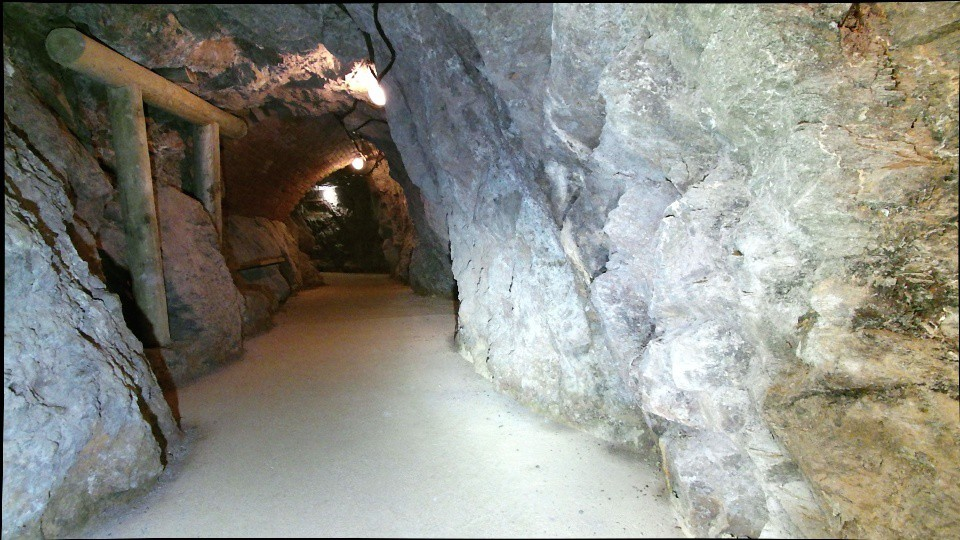
\includegraphics[width=0.5\linewidth]{chapter05/img/lehrpfad/color0000.jpg}%
    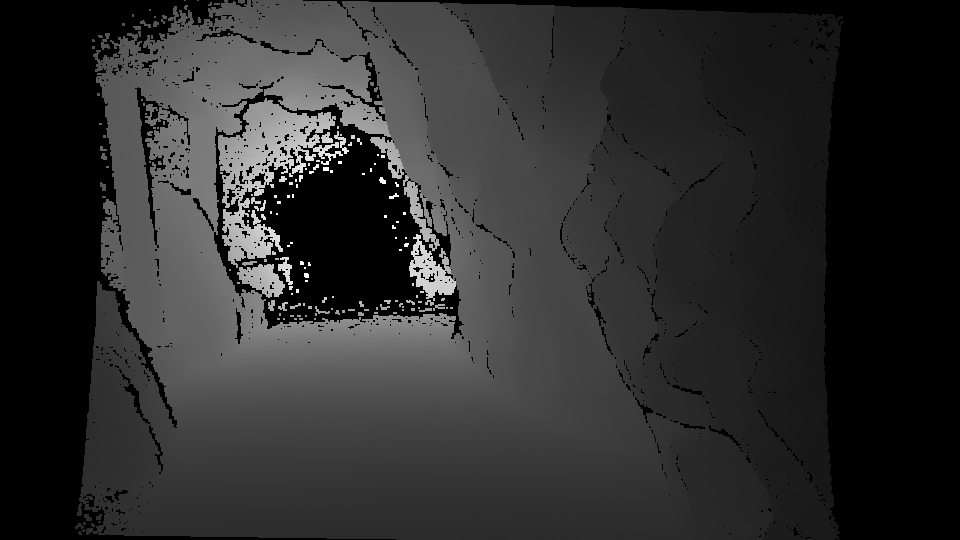
\includegraphics[width=0.5\linewidth]{chapter05/img/lehrpfad/depth-scaled-0000.png}\\
    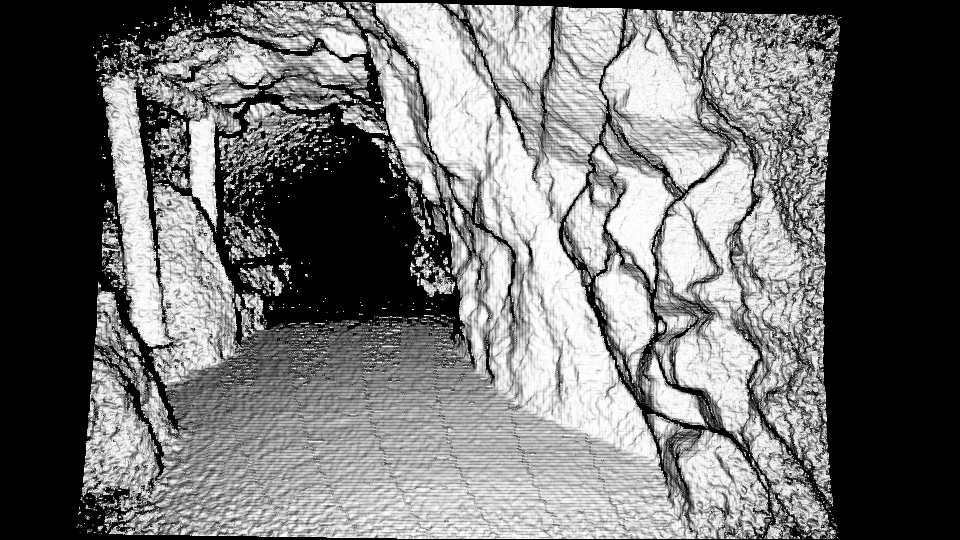
\includegraphics[width=0.5\linewidth]{chapter05/img/lehrpfad/flexion-0000.png}%
    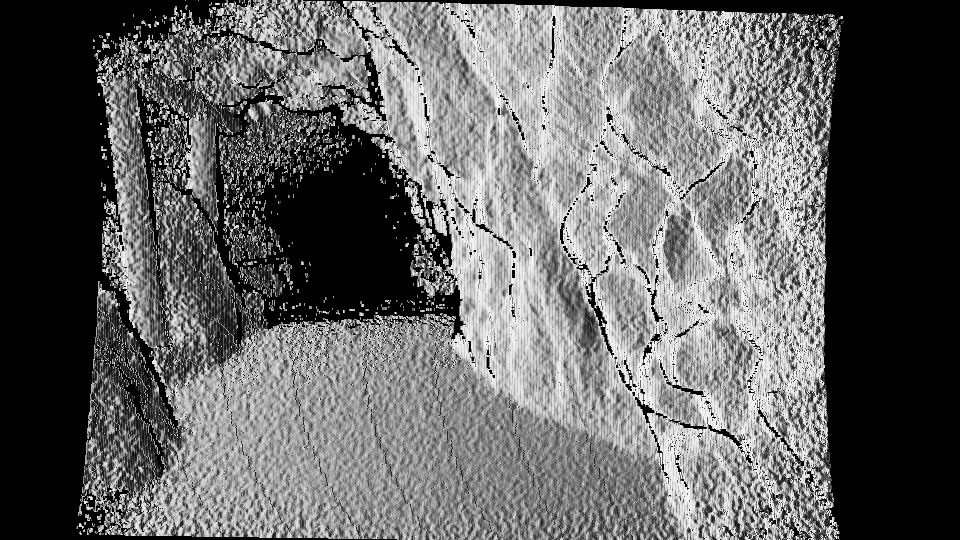
\includegraphics[width=0.5\linewidth]{chapter05/img/lehrpfad/bearing-0000.png}%
    }
    {\caption{Images of the \emph{Mine} dataset.}\label{fig:lehrpfad_data}}
\end{floatrow}
\end{figure}

\subsubsection{Office}

The second Kinectv2 dataset is taken in an office with many smaller elements, wires and other manmade objects.
It contains 57 images composed of translation and rotation of the depth sensor (example images in Appendix~\ref{sec:office_conversions}).
No trajectory reconstruction other than the ICP is used for the relative poses.
It contains similar measurement errors as the Mine dataset, but has more distinctive shapes and better overall conditions for the depth sensor.
\begin{figure}[H]
\CenterFloatBoxes%
\begin{floatrow}
    \btabbox{%
    \renewcommand{\arraystretch}{1.2}%
    \setlength{\tabcolsep}{1em}%
    \begin{tabular}{rc}
    \toprule
    \textbf{Parameter} & \textbf{Kinectv2} \\
    \midrule
    Principle  & pinhole \\
    Resolution & 960 $\times$ 540\,px \\
    $f_x$, $f_y$ & 519.23, 522.23 \\
    $c_x$, $c_y$ &  479.46, 272.74 \\
    \bottomrule
    \end{tabular}}
    {\caption{Office Kinectv2 intrinsic.}\label{tab:office_intrinsic}}%
    \ffigbox{%
    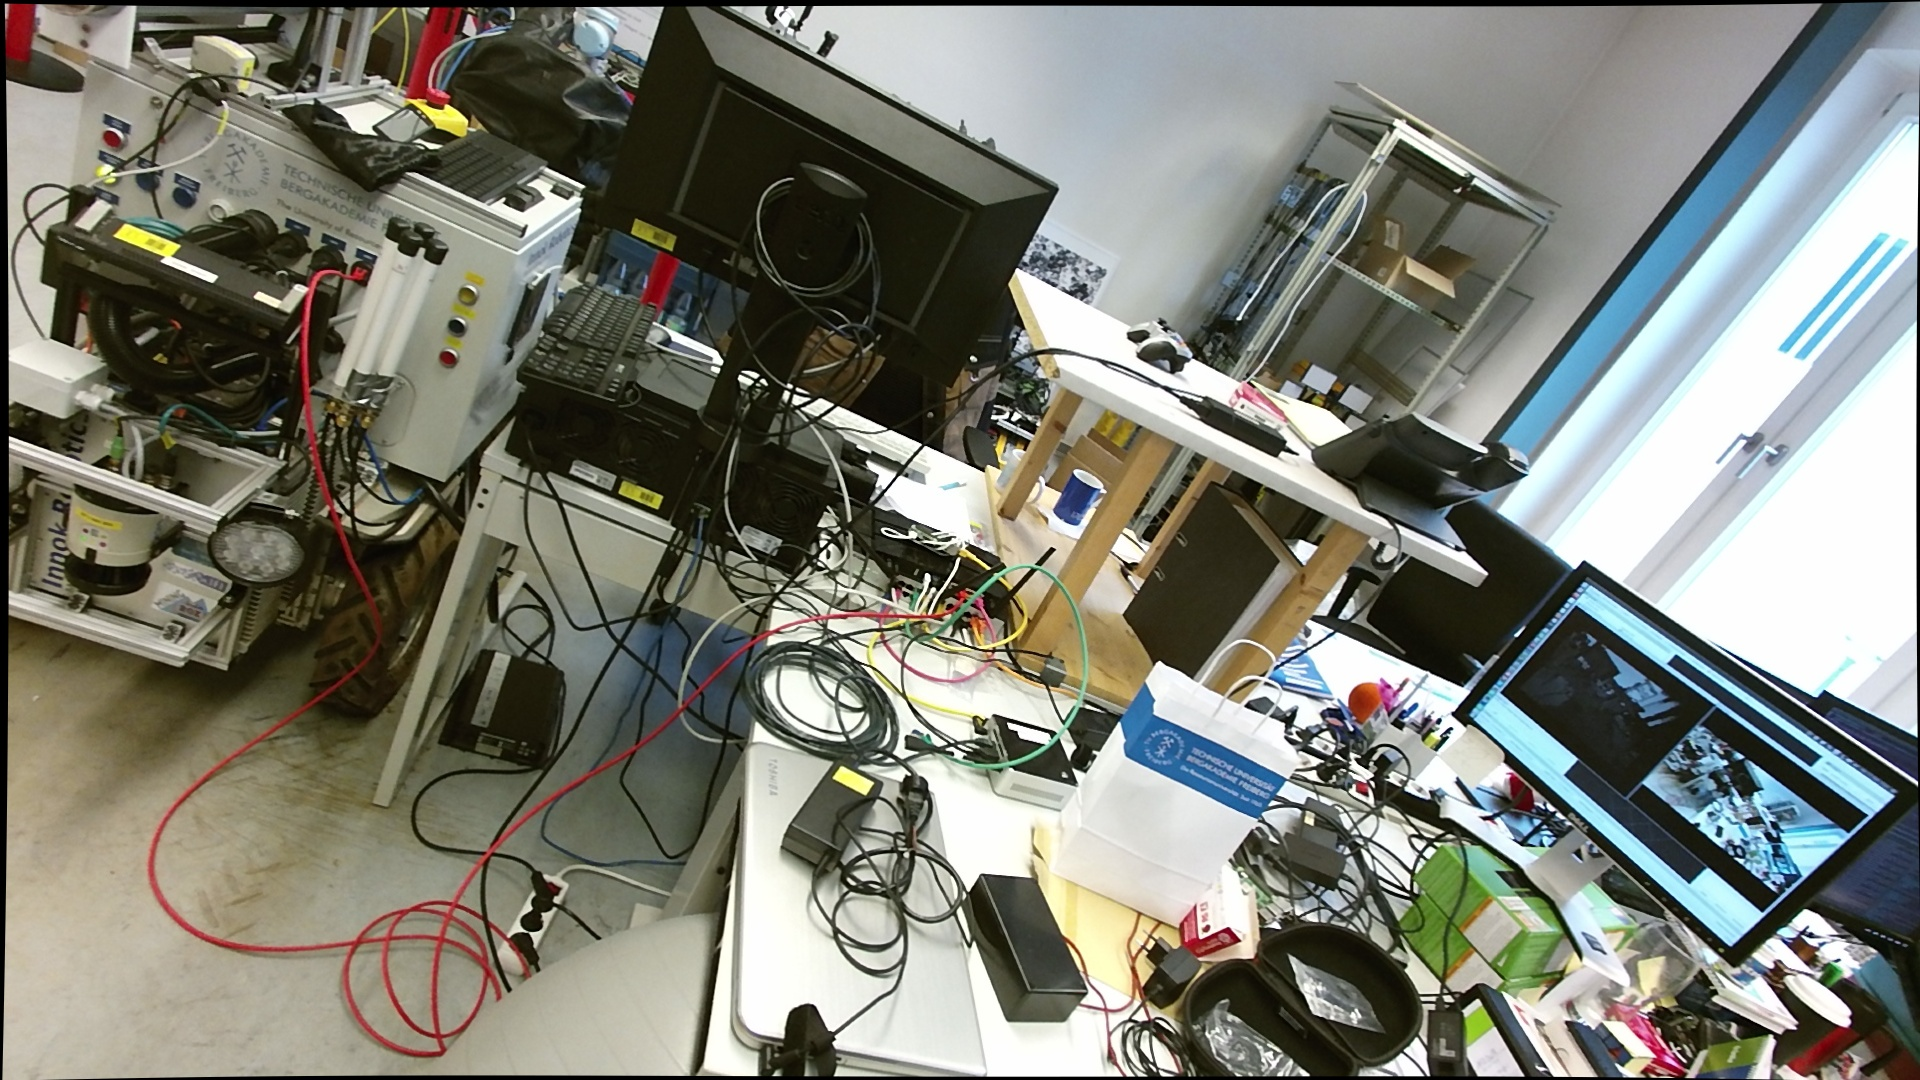
\includegraphics[width=0.5\linewidth]{chapter05/img/office/color_0024.jpg}%
    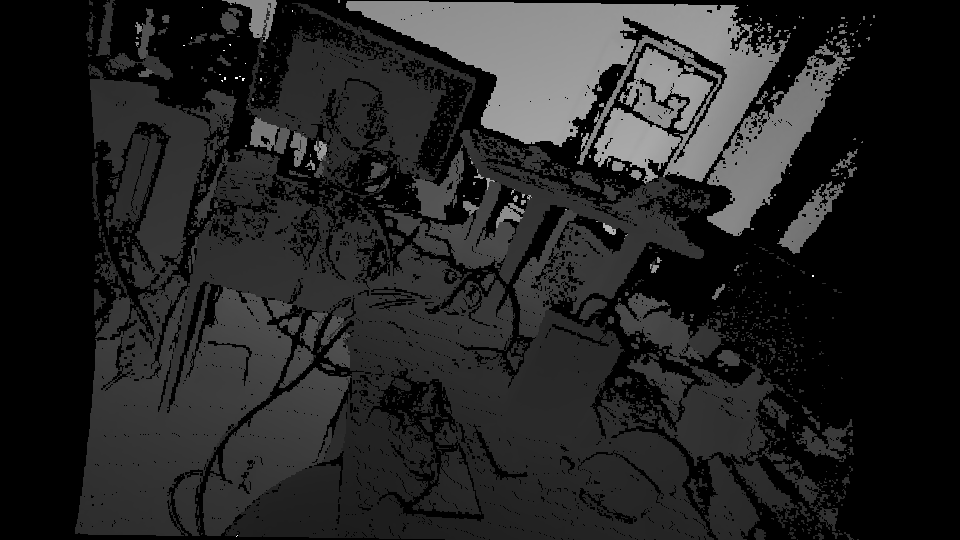
\includegraphics[width=0.5\linewidth]{chapter05/img/office/depth_scaled_0024.png}\\
    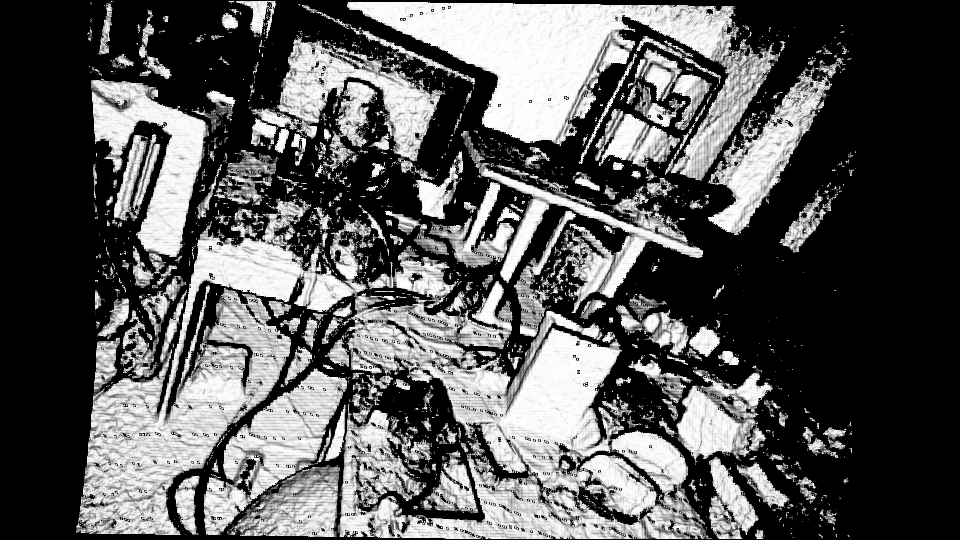
\includegraphics[width=0.5\linewidth]{chapter05/img/office/flexion_0024.png}%
    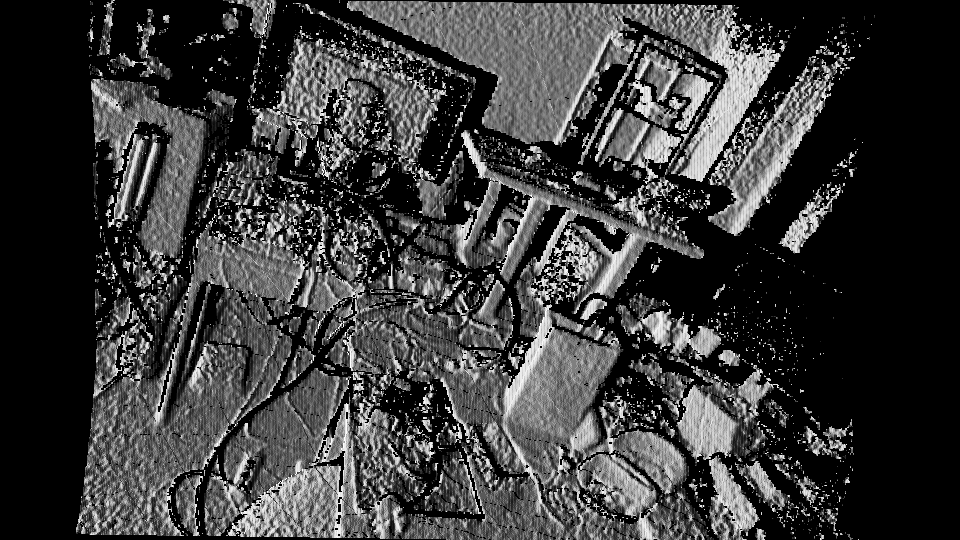
\includegraphics[width=0.5\linewidth]{chapter05/img/office/bearing_0024.png}%
    }
    {\caption{Images of the \emph{Office} dataset.}\label{fig:office_data}}
\end{floatrow}
\end{figure}

\subsubsection{Laserscan}

Full \acrshort{LIDAR} scans are taken as part of classical mine surveying in the Reiche Zeche.
The scans were done in the section \emph{Wilhelm-Stehender-Süd} of the mine.
These scans are examined for the conversions, too.
Because they were done with classical artificial marker based registration in mind, the overlap between those scans is minimal.
This unfortunatly means, that a direct matching between scans is meaningless.
The distribution and characteristics of the extracted features is analyzed, though.
From the raw dataset only 6 scans are selected, because each scan had a slightly different resolution and aspect ratio (example scans in Appendix~\ref{sec:laserscan_conversions}).
The selected scans were manually processed to have a common resolution and aspect ratio.
\begin{figure}[H]
\CenterFloatBoxes%
\begin{floatrow}
    \btabbox{%
    \renewcommand{\arraystretch}{1.2}%
    \setlength{\tabcolsep}{1em}%
    \begin{tabular}{rc}
    \toprule
    \textbf{Parameter} & \textbf{Riegl Z300} \\
    \midrule
    Principle  & equirectangular \\
    Resolution & 3600 $\times$ 800\,px \\
    $\theta_{min}$, $\theta_{max}$ & \shortstack{0.87, 2.27 \\ (49.85\degree, 130.06\degree)} \\
    \bottomrule
    \end{tabular}}
    {\caption{Riegl Z300 \acrshort{LIDAR} intrinsic.}\label{tab:scan_intrinsic}}%
    \ffigbox{%
    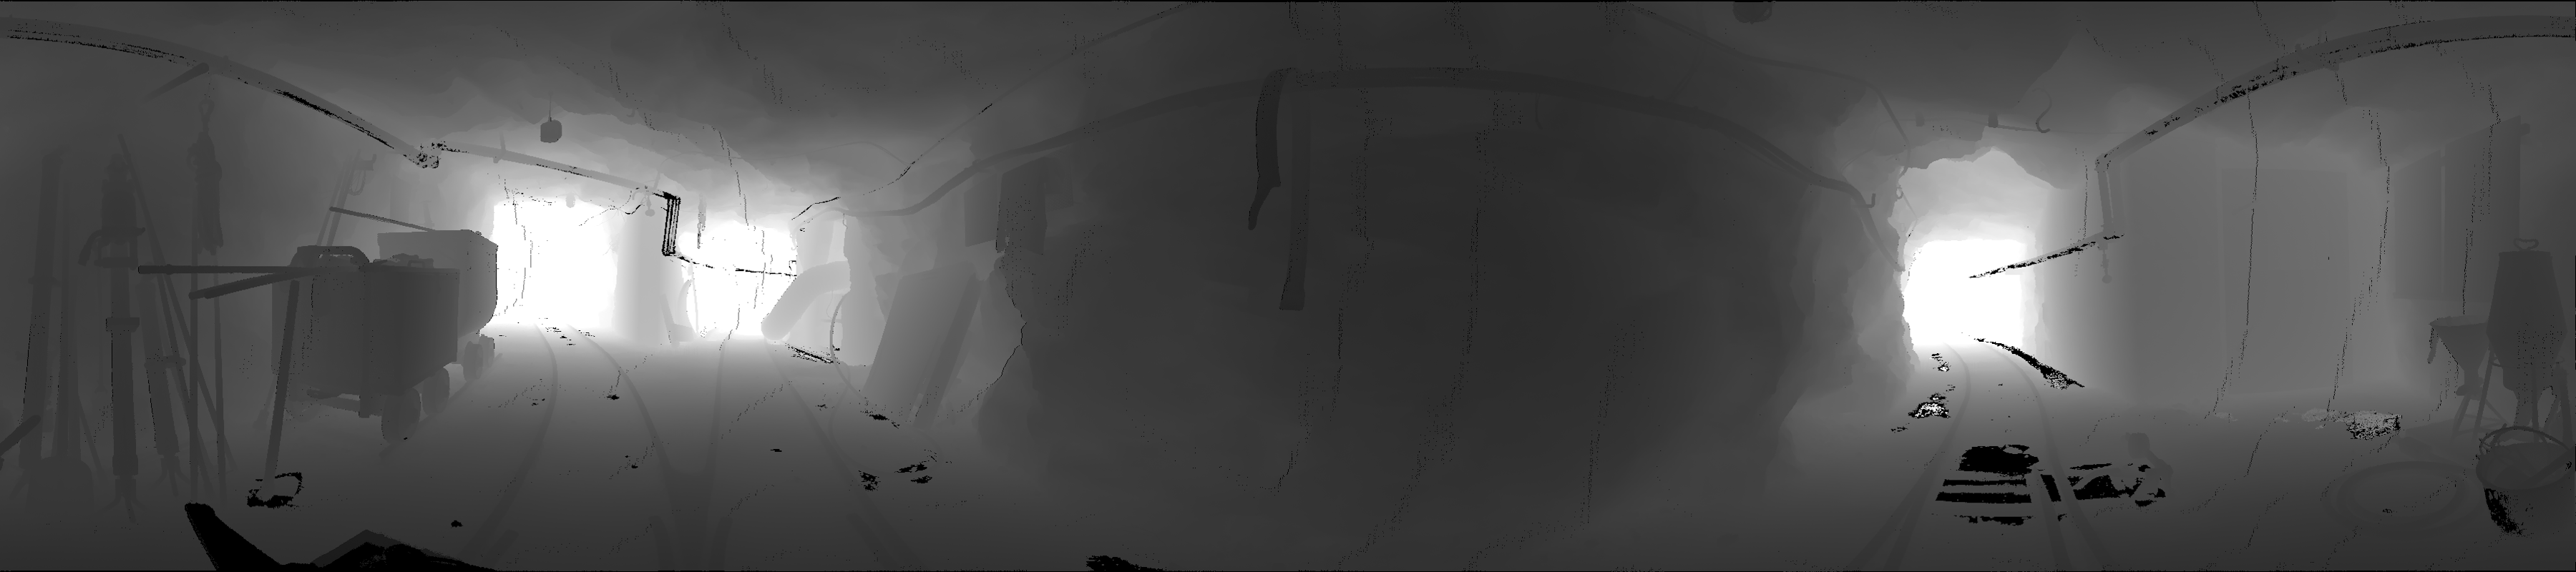
\includegraphics[width=1\linewidth]{chapter05/img/scans/range-0001.png}\\
    
\includegraphics[width=1\linewidth]{chapter05/img/scans/flexion-0001.png}\\
    \includegraphics[width=1\linewidth]{chapter05/img/scans/bearing-0001.png}%
    }
    {\caption{The raw \acrshort{LIDAR} scans and their conversions.}\label{fig:scans}}
\end{floatrow}
\end{figure}

\begin{table}[H]
    {\renewcommand{\arraystretch}{1.3}%
    \setlength{\tabcolsep}{0.3em}%
    \begin{tabular}{ccccc}
    \toprule
    \null & \textbf{Synthetic} & \textbf{Mine} & \textbf{Office} & \textbf{Laserscan} \\
    \midrule
    \textbf{Camera Model} & pinhole & pinhole & pinhole & equirectangular \\
    \textbf{Number Images} & 211 & 734 & 57 & 6 \\
    \textbf{Distribution} & \ding{52} & \ding{52} & \ding{52} & \ding{52} \\
    \textbf{Keypoint Characteristics} & \ding{52} & \ding{52} & \ding{52} & \ding{52} \\
    \textbf{Matching Performance} & \ding{52} & \ding{52} & \ding{52} & \ding{56} \\
    \bottomrule
    \end{tabular}
    }
    \caption{An overview of all datasets and aspects of them were analyzed.}
\end{table}

\subsubsection{Synthetic City Scene Odometry}

The datasets presented before evaluate the feature algorithms and show their potential and performance.
To demonstrate, that the results are applicable in other scenarios, the most promising algorithms are used to compute a visual odometry.
A synthetic city dataset, developed by Zhang et al.\cite{zhang_icra2016}, that provides a groundthruth trajectory serves as test.
The in-house visual odometry implementation, based on Singh's\cite{singh_report2015} work, is very basic with the following four steps.
First, the features are detected and their descriptors extracted.
The descriptors are matched.
The essential matrix is computed using RANSAC and the consensus pose is used as relative pose.
Each feature algorithm is executed with its default configuration.
Both conditions imply that the result is not optimal and further optimizations would improve it further.
